\documentclass{llncs}
\usepackage[latin1]{inputenc}
%\usepackage[T1]{fontenc}
%\usepackage{textcomp}
\usepackage{graphicx}
\usepackage{color}
%\usepackage{setspace}
\usepackage{url}
\usepackage[english]{babel}


\begin{document}

%%%%%%%%%%%%%%%%%%%%%%%%%%%%%%%   TITLE   %%%%%%%%%%%%%%%%%%%%%%%%%%%%%%%

\title{Visualizaci�n de Programas Gamificada}

%%%%%%%%%%%%%%%%%%%%%%%%%%%%%%%   AUTHORS   %%%%%%%%%%%%%%%%%%%%%%%%%%%%%%%

\author{R.M. Hidalgo-Berm�dez, M.S. Rodr�guez-Domingo, A.M. Mora,\\ P. Garc�a-S�nchez, J.J. Merelo}
\authorrunning{R.M. Hidalgo et al.}

\institute{
Departamento de Arquitectura y Tecnolog�a de Computadores. \\
Escuela T�cnica Superior de Ingenier�as Inform�tica y de Telecomunicaci�n. \\
University of Granada, Spain \\
\email{rosa.hb84@gmail.com, zandra@correo.ugr.es\\ \{amorag,pgarcia,jmerelo\}@geneura.ugr.es}
}

\maketitle

%
%%%%%%%%%%%%%%%%%%%%%%%%%%%%%%%%%   ABSTRACT   %%%%%%%%%%%%%%%%%%%%%%%%%%%%%%%%%
%
\begin{abstract} 
All throughout their history, video games have considerably evolved from their original shape to what they have become now: complex technological products creating a massive industry and market as important as that of the cinematographic one. 
Most of game development has been focused on the technical part (graphics and sound), leaving the artificial intelligence aside. However, artificial intelligence and specifically computational intelligence is becoming more significant, leading to much research on how to provide non-playing characters  with adapted and unpredictable behaviour so as to afford users a better gaming experience.
This work applies strategies based on Genetic Algorithms mixed with behavioural models, to obtain an agent (or bot) capable of completing autonomously different scenarios on a simulator of Super Mario Bros. game.
Specifically, the agent follows the rules of the \textit{Gameplay} track of Mario AI Championship.
Different approaches have been analyzed, combining Genetic Algorithms with Finite State Machines, yielding agents which can complete levels of different difficulties playing much better than an expert human player.
\end{abstract}


%\textbf{Keywords.} Video Games, Super Mario Bros, Genetic Algorithms,
%Artificial Intelligence, Non Player Character, Finite State Machine

%
%%%%%%%%%%%%%%%%%%%%%%%%%%%%%%%   INTRODUCTION   %%%%%%%%%%%%%%%%%%%%%%%%%%%%%%%
%
\section{Introduction}
\label{sec:intro}

First modern video games appeared in the 60s, and since then, this area has not stopped growing. In 1981, Shigeru Miyamoto\footnote{Designer and producer of Nintendo Ltd., and winner of the 2012 Pr�ncipe de Asturias Prize in Humanities and Communication} created Donkey Kong, in which a plumber named Jumpman tries to rescue his girlfriend from a gorilla's. This character was evolved, and in 1983 (thanks again to Shigeru Miyamoto) Mario Bros. games series appeared. The most famous was platform game Super Mario Bros., which was launched in arcade and also in the Nintendo's home console NES. Several other sequels have been published, including the blockbuster Super Mario World in the 90s, which presented a great improvement in graphics, sound and playability.

All of them follow the same plot: the plumber Mario must rescue the princess of Mushroom Kingdom, Peach, who has been kidnapped by the king of the koopas, Bowser. The main goal is to go across lateral platforming levels, trying to avoid different types of enemies and obstacles and using some useful (but limited) items, such as mushrooms or fire flowers. 

Due to their success, amusement and attractiveness, videogames have become one of the most extended research areas regarding the Artificial Intelligence (AI) field, yielding the so-called Computational Intelligence (CI) branch. Several games have become extended frameworks for study new techniques and algorithms in these scopes, such as Quake \cite{laird2001using}, Unreal \cite{Agent_Smith_CEC2009,cooperativebots_CIG2010}, Pac-Man \cite{Pac-MAnt_CIG2010,MTCS_PacMan}, Starcraft \cite{starcraft_bayesianmodel,potfields_starcraft} and, of course, Super Mario Bros. \cite{SuperMario_playerexperience,SuperMario_Togelius,SuperMario_rulebased,SuperMario_levelgeneration}.

The framework developed for the latter is Mario AI, a modified version of the game known as Infinite Mario Bros.\footnote{\email{http://www.mojang.com/notch/mario/}}, an open-code application where the researchers can implement, for instance interactive and autonomous behavioural routines, using the set of functions and variables it offers.
Moreover, in order to motivate the scientific community to perform these studies, a competition is proposed three times a year, inside several famous conferences, it is called the \textit{Mario AI Championship}\footnote{\email{http://www.marioai.org/}}, and is composed by some tracks: Learning, Level generation, Turing test, and Gameplay.
The latter is devoted to create the best autonomous agent (also known as bot) as possible for automatically playing and pass sequential levels with a growing difficulty.

This work presents different approaches of autonomous agents, which follow the behaviour modelled by means of a finite state machine (FSM) \cite{FSM_Booth}. This behavioural engine, based on expert knowledge, has been improved by applying offline (not during game) optimization using evolutionary algorithms (EAs) \cite{EAs_Back96}, considering different schemes.

The two approaches have been widely tested and analyzed, getting an optimal set of parameters for the EA and thus, very competent agents in a number of difficulty levels.

The rest of the paper is organized as follows. Next section presents some preliminary concepts and background of the work. Section \ref{sec:environment} defines the problem itself, describing the competition rules, along with the Infinite Mario Bros. platform, regarding the main features that the agent must consider and its constraints. Then, Section \ref{sec:FSMagent} introduces the agents' approaches which will be analyzed in the paper, along with the set of experiments conducted to perform this analysis (Section \ref{sec:experiments}). Finally, Section \ref{sec:conclusions} describes the reached conclusions.

%
%%%%%%%%%%%%%%%%%%%%%%%%%%%%%%%   BACKGROUND  %%%%%%%%%%%%%%%%%%%%%%%%%%%%%%%
%
\section{Preliminary concepts and background}
\label{sec:preliminaryconcepts}

In this section, the main techniques applied in the development of this work are briefly described.

%----------------------------------------------------------------------------
\subsection{Genetic Algorithms}
\label{subsec:GAs}

Evolutionary Algorithms (EAs) are a class of direct, probabilistic search and optimization algorithms gleaned from the model of darwinistic evolution \cite{EAs_Back96}. They have been widely used for solving combinatorial and optimization problems. 
%An EA works with population of possible solutions (individuals) for the target problem, a selection method that favours better solutions and a set of operators that act upon the selected solutions. After an initial population is created (usually randomly), the selection and operators are successively applied to the individuals in order to create new populations that replace the older one. This process guarantees that the average quality of the individuals tends to increase with the number of generations. Eventually, depending on the type of problem and on the efficiency of the EA, an optimal solution may be found.
The most extended class of EA are the Genetic Algorithms (GAs) \cite{GAs_Goldberg89}. A GA is composed of a \textit{population of candidate solutions} to a problem that evolve towards optimal (local or global) points of the search space by recombining parts of the solutions to generate a new population. The decision variables of the problem are encoded in strings with a certain length and cardinality. In GAs' terminology, these strings are referred to as \textit{chromosomes}, each string position is a \textit{gene} and its values are the \textit{alleles}. The alleles may be binary, integer, real-valued, etc, depending on the codification (which in turn may depend on the type of problem). 
As stated, the ``best'' parts of the chromosomes (or building-blocks) are guaranteed to spread across the population by a \textit{selection mechanism} that favours better (or fitter) solutions. The quality of the solutions is evaluated by computing the \textit{fitness} values of the chromosomes; this fitness function is usually the only information given to the GA about the problem. 
A standard GA's procedure is shown in Figure \ref{fig:GA_pseudocode}.

\begin{figure}[ht]
\begin{center}
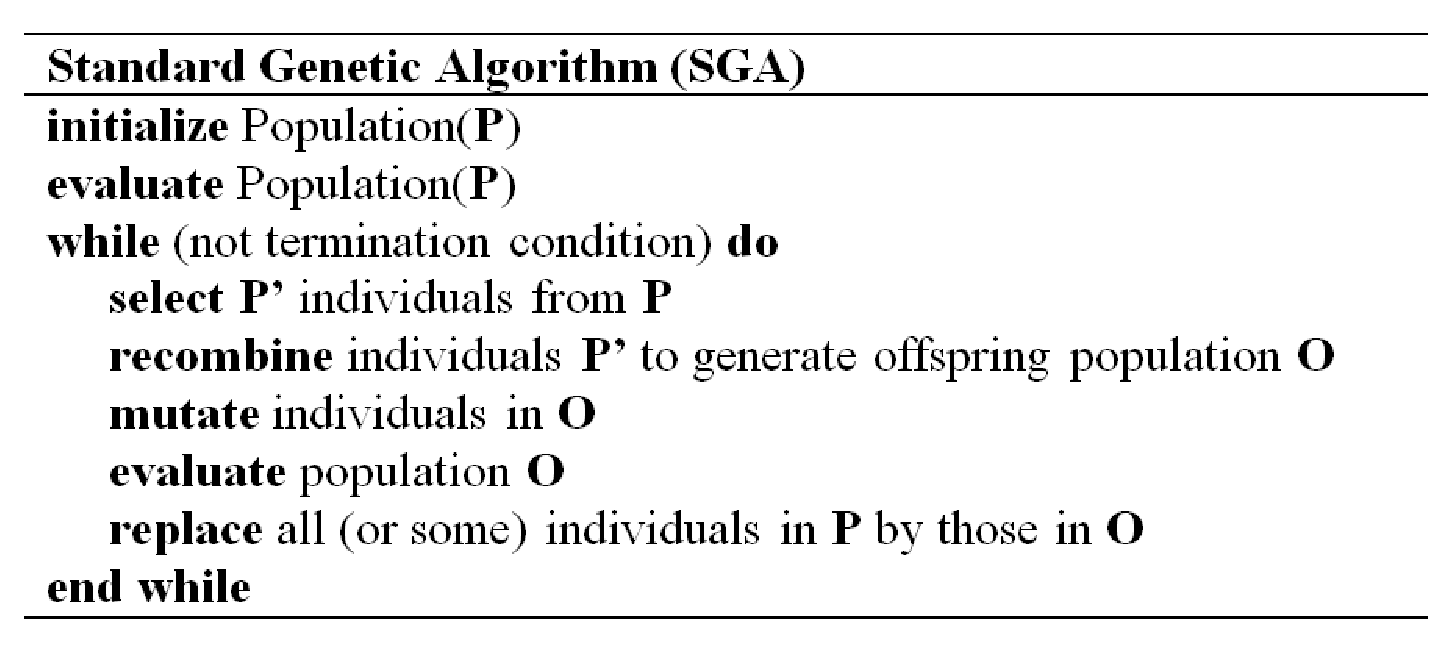
\includegraphics[scale=0.45]{imags/GA_pseudocode.eps}
\caption{Standard GA pseudocode.
\label{fig:GA_pseudocode}}
\end{center}
\end{figure}

It works as follows: First, a population of chromosomes is randomly generated. All the chromosomes in the population are then evaluated according to the fitness function. A pool of parents (or mating pool) is selected by a method that guarantees that fitter individuals have a better chance of being in the pool. After selection, a new population is generated by recombining the genes in the parents' population. This is usually done with a crossover operator (1-point crossover, or uniform crossover, amongst many proposals that can be found in the Evolutionary Computation literature) that recombines the genes of two parents and generates two offspring according to a crossover probability. Then, once the offspring population is complete, the new chromosomes are mutated before being evaluated by the fitness function. Mutation operates at gene level considering a probability (which is usually very low).
After the evaluation of the offspring population the algorithm starts the replacement of the old population, following a specific policy. Generational replacement, for instance, replaces the old population by the offspring. A steady-state strategy, on the other hand, will replace a fraction (typically, two individuals) of the old population by the best individuals in the offspring population. Normally, an $e$-elitism strategy is used, i.e., the best $e$ chromosomes from the old population are copied without mutation to the new population. The remaining individuals are selected according to any method. 
This process goes on until a stop criterion is met. Then, the best individual in the population is retrieved as a possible solution to the problem. 

EAs have been applied in a wide range of optimization problems, including in recent years (10 years ago) their application in videogames area \cite{optimalRTS,tactics_evolutionary_learning,SuperMario_Togelius,Agent_Smith_CEC2009,cooperativebots_CIG2010}. The problem is they usually involve considerable computational cost and thus they are not frequently used in on-line games. In fact, the most successful proposals for using EAs in games correspond to off-line applications \cite{evolutionary_learning-offline}, that is, the EA works (for instance, to improve the operational rules that guide the bot's actions) while the game is not being played, and the results or improvements can be used later during the game. Through offline evolutionary learning, the quality of bots' intelligence in commercial games can be improved, and this has been proven to be more effective than opponent-based scripts.
This way, in this work, an offline EA is applied to a parameterized behavioural model for a Super Mario agent, in order to improve its decision engine, which will be used later during game (online).

%----------------------------------------------------------------------------
\subsection{Finite State Machines}
\label{subsec:FSMs}

A Finite State Machine (FSM) \cite{FSM_Booth} or Finite State Automaton is a computational model which represents a set of \textit{states} and connections between them. Every connection correspond to a \textit{transition} from one state to another one, depending on the state inputs and the so-called transition function.

It is represented as a directed graph, where the states are nodes labelled with a name, and the transitions are edges with an associated value representing the input that should be received to move between states through this transition. The graph can be connected at different degrees (is not always fully connected), depending on the possible transitions to model.

There is usually an initial state, where the model starts working, and a final state, which is the final output of the automaton.

FSMs were initially designed to recognise regular and formal languages, but nowadays they are used as a powerful behaviour modelling tool inside videogames, i.e., the AI of an autonomous character can be defined by means of a FSM. 
They are based in \textit{sensors}, which receive environmental inputs and \textit{actuators}, which perform the response actions to these inputs. In the FSM model, the possible values received by the sensors are set in the edges of the graph (as transitions), meanwhile the actuators' actions happen in every state.
Several videogames have implemented this technique, from Pac-Man (modelling the ghosts' behaviour) to Unreal Tournament series, which is one of the best considered games regarding its Bots (agents) AI.

In the present work, the behavioural model for our Mario agent has been implemented by means of a FSM, since it can easily model (or simulate) the behaviour of an expert player.


%%%%%%%%%%%%%%%%%%%%%%%%%%%%%  ENVIRONMENT %%%%%%%%%%%%%%%%%%%%%%%%%%%%%%%%

\section{Mario AI: Competition and Environment}
\label{sec:environment}

%\subsection{The Competition}
%\label{subsec:competition}

The proposed agents follow the rules of the Mario AI Championship\footnote{\email{http://www.marioai.org/}} devoted to address different CI tasks (content generation, learning, autonomous agents and Turing test).

Specifically, Mario AI is a simulator, a version of Infinite Mario Bros., which is available in open code and make it easier for the competitors to implement their algorithms, using a set of classes, variables and high-level functions.
It includes a wide support for implementing autonomous agents to control Mario character using AI techniques.

The competition consists of four categories: 
\begin{itemize}
    \item Gameplay: looking for the best Mario agent (bot), i.e. the one who can pass a higher amount of levels with growing difficulty.
    \item Learning: the agent must learn to play a particular level in a limited time.
    \item Level Generation: generation of levels which should be as fun as possible (according to human players).
    \item Turing Test: the agent must behave as a human.
\end{itemize}

Even being a relatively new competition, it has already been quite successful and had numerous participants with very interesting results and algorithms. Such as the work by Bojarski and Bates-Congdon, called REALM \cite{SuperMario_rulebased}, in which an agent based on a evolutionary set of rules is developed, specifying some goals to achieve starting from a set of conditions and actions. This agent won the competition in the categories of GamePlay and Learning in the CIG 2010 edition.

In the category of GamePlay the main goal is to complete as many levels as posible. The problem can be interpreted as a pathfinding one, as Baumgarten \cite{SuperMario_Astar} did. They solve the objective of finding the fastest way through the surroundings in which Mario stays alive by using an A* searching. This algorithm has proved to be quick and flexible enough to find routes through the levels generated even in real time.

Our aim was to implement an intelligent agent which could compete in the GamePlay track. In order to do this, we have applied GAs along with behavioural models (set of rules and a FSM).
The choice of Genetic Algorithms is due to its adaptability, as with them we do not need specific knowledge of the problem that we want to solve; they operate with diverse simultaneous solutions to the problem and they allow to optimize the solution of the problem with regard to different goals. Even though its convergence will not be as fast as that of other more specific algorithms for the problem that we want to tackle, in most of the cases we will find a solution that, even though it is not the best possible, it will be the best for the pre-established aims.


%\subsection{The Environment}
%\label{subsec:environment}

The game consists in moving the character, Mario, through bi-dimensional levels. He can move left and right, down (crouch), run (letting the button pushed), jump and shoot fireballs (when in ``fire'' mode).

The main goal is complete the level, whereas secondary goals could be  killing enemies and collecting coins or other items. These items may be hidden and may cause Mario to change his state (for instance a fire flower placed `inside' a block).
The difficulty of the game lies in the presence of cliffs/gaps and enemies. Mario loses power (i.e., its status goes down one level) when touched by an enemy and dies if he falls off a cliff. Figure \ref{fig:level_example} shows a screen capture of the game.

\begin{figure}
\begin{center}
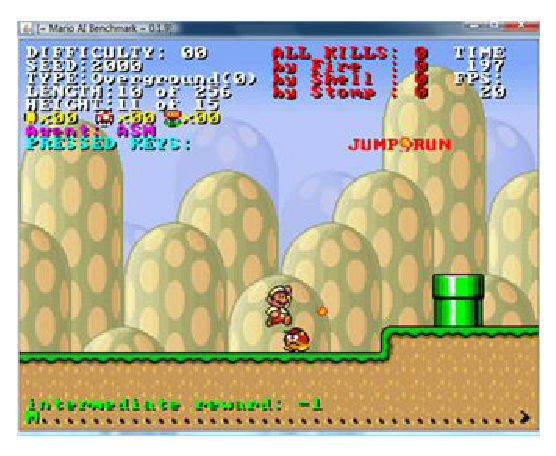
\includegraphics[scale=0.8]{imags/level_example.eps}
\caption{Infinite Mario screen capture showing a level, and the information provided by the Mario AI simulator.
\label{fig:level_example}}
\end{center}
\end{figure}

Mario can be in three different modes:

\begin{itemize}
\item {\em Small}: In this mode Mario is smaller than in the others. If an enemy strikes him, Mario dies. He can't crouch.
\item {\em Big}: This is Mario's intermediate mode. Mario reaches this mode if he is in Fire state and an enemy touches him, or devouring a mushroom in the Small state.
\item {\em Fire}: In it Mario can shoot fireballs. Mario can reach this mode if he is in Big mode and takes a fire flower.
\end{itemize}

The simulator provides information about Mario's surrounding areas. According to the rules of the competition, two matrixes give this information, both of them are 19x19 cells size, centred in Mario. One contains the positions of surrounding enemies, and the other provides information about the objects in the area (scenery objects and items).

Every tick (40 ms), Mario's next \textit{action} must be indicated. This action consist in a combination of the five possible movements that Mario can do (left, right, down, fire/speed, jump). This information is encoded into a boolean array, containing a 1 value when a movement must be done.

The action to perform depends, of course, in the scenery characteristics around Mario, but it is also important to know where the enemies are and their type. Thus, the agent could know if it is best to jump, shoot or avoid them. We have defined four main enemies groups according to what the agent needs to do to neutralize them: one for enemies who die by a fireball/jump/Koopa shell, other for those who only die by a fireball, others which only die jumping on them, and finally others which just die by a Koopa shell.

%\begin{itemize}
%\item Enemies who can die by a fireball strike or if Mario jumps on them and crushes them or if Mario is carrying a koopa shell and throws it at the enemies: Goomba, Goomba Windged, Green Koopa, Red Koopa, Koopa Windged Green, Red Koopa Windged.
%
%\item Enemies who only die by a fireball strike: carnivorous flowers that appear in the pipes.
%
%\item Enemies who only die when Mario jumps on them and crushes them: the cannon balls.
%
%\item Enemies who only die if Mario launches a koopa shell against them: the Spiky and Spiky Windged\\\\
%\end{itemize}


%%%%%%%%%%%%%%%%%%%%%%%%%%%%%  AGENT DESIGN %%%%%%%%%%%%%%%%%%%%%%%%%%%%%%%%

\section{Evolutionary FSM-based Agent}
\label{sec:FSMagent}

The proposed agent, \textit{evoFSM-Mario}, is based in a FSM which models a logical behaviour, and which has been designed following an expert player knowledge.
We decided to combine this technique with EAs, since they have proved being an excellent adapting and optimization method, very useful for improving predefined behavioural rules, as the FSMs model.

We have defined a table of possible states for the agent, including all the possible (valid) actions the agent can perform in a specific instant, i.e. feasible combinations of moving left, moving right, crouch (going down), jump and fire/run.
Table \ref{tab:FSMstates} shows the codification of the states in boolean values.

%\begin{table} [htbp]
%\centering
%{\small
%\begin{tabular}{|l|l|l|l|l|l|}
%\cline{2-6}
%\multicolumn{1}{l|}{} & \multicolumn{1}{c|}{Right} & \multicolumn{1}{c|}{Left} & \multicolumn{1}{c|}{Fire/Run} & \multicolumn{1}{c|}{Jump} & \multicolumn{1}{c|}{Down} \\ 
%\hline
%\textit{State 0} & \multicolumn{1}{c|}{1} & \multicolumn{1}{c|}{0} & \multicolumn{1}{c|}{0} & \multicolumn{1}{c|}{0} & \multicolumn{1}{c|}{0} \\ 
%\hline
%\textit{State 1} & \multicolumn{1}{c|}{1} & \multicolumn{1}{c|}{0} & \multicolumn{1}{c|}{0} & \multicolumn{1}{c|}{1} & \multicolumn{1}{c|}{0} \\ 
%\hline
%\textit{State 2} & \multicolumn{1}{c|}{1} & \multicolumn{1}{c|}{0} & \multicolumn{1}{c|}{1} & \multicolumn{1}{c|}{0} & \multicolumn{1}{c|}{0} \\ 
%\hline
%\textit{State 3} & \multicolumn{1}{c|}{1} & \multicolumn{1}{c|}{0} & \multicolumn{1}{c|}{1} & \multicolumn{1}{c|}{1} & \multicolumn{1}{c|}{0} \\ 
%\hline
%\textit{State 4} & \multicolumn{1}{c|}{0} & \multicolumn{1}{c|}{1} & \multicolumn{1}{c|}{0} & \multicolumn{1}{c|}{0} & \multicolumn{1}{c|}{0} \\ 
%\hline
%\textit{State 5} & \multicolumn{1}{c|}{0} & \multicolumn{1}{c|}{1} & \multicolumn{1}{c|}{0} & \multicolumn{1}{c|}{1} & \multicolumn{1}{c|}{0} \\ 
%\hline
%\textit{State 6} & \multicolumn{1}{c|}{0} & \multicolumn{1}{c|}{1} & \multicolumn{1}{c|}{1} & \multicolumn{1}{c|}{0} & \multicolumn{1}{c|}{0} \\ 
%\hline
%\textit{State 7} & \multicolumn{1}{c|}{0} & \multicolumn{1}{c|}{1} & \multicolumn{1}{c|}{1} & \multicolumn{1}{c|}{1} & \multicolumn{1}{c|}{0} \\ 
%\hline
%\textit{State 8} & \multicolumn{1}{c|}{0} & \multicolumn{1}{c|}{0} & \multicolumn{1}{c|}{0} & \multicolumn{1}{c|}{0} & \multicolumn{1}{c|}{0} \\ 
%\hline
%\textit{State 9} & \multicolumn{1}{c|}{0} & \multicolumn{1}{c|}{0} & \multicolumn{1}{c|}{0} & \multicolumn{1}{c|}{0} & \multicolumn{1}{c|}{1} \\ 
%\hline
%\textit{State 10} & \multicolumn{1}{c|}{0} & \multicolumn{1}{c|}{0} & \multicolumn{1}{c|}{0} & \multicolumn{1}{c|}{1} & \multicolumn{1}{c|}{0} \\ 
%\hline
%\textit{State 11} & \multicolumn{1}{c|}{0} & \multicolumn{1}{c|}{0} & \multicolumn{1}{c|}{0} & \multicolumn{1}{c|}{1} & \multicolumn{1}{c|}{1} \\ 
%\hline
%\textit{State 12} & \multicolumn{1}{c|}{0} & \multicolumn{1}{c|}{0} & \multicolumn{1}{c|}{1} & \multicolumn{1}{c|}{0} & \multicolumn{1}{c|}{0} \\ 
%\hline
%\textit{State 13} & \multicolumn{1}{c|}{0} & \multicolumn{1}{c|}{0} & \multicolumn{1}{c|}{1} & \multicolumn{1}{c|}{1} & \multicolumn{1}{c|}{0} \\ 
%\hline
%\end{tabular}
%}
%\caption{Codification of the feasible states of the FSM which will model the Mario agent's AI. 1 is $true/active$, 0 is $false/non-active$.
%\label{tab:FSMstates} }
%\end{table}

\begin{table} [htbp]
\centering
{\footnotesize
\begin{tabular}{|c|c|c|c|c|c|c|c|c|c|c|c|c|c|c|}
\hline
& \textit{St 0}  & \textit{St 1} & \textit{St 2} & \textit{St 3} & \textit{St 4} & \textit{St 5} & \textit{St 6} & \textit{St 7} & \textit{St 8} & \textit{St 9} & \textit{St 10} & \textit{St 11} & \textit{St 12} & \textit{St 13}\\
\hline
Right & 1 & 1 & 1 & 1 & 0 & 0 & 0 & 0 & 0 & 0 & 0 & 0 & 0 & 0\\
\hline
Left & 0 & 0 & 0 & 0 & 1 & 1 & 1 & 1 & 0 & 0 & 0 & 0 & 0 & 0\\
\hline
Fire/Run & 0 & 0 & 1 & 1 & 0 & 0 & 1 & 1 & 0 & 0 & 0 & 0 & 1 & 1\\
\hline
Jump & 0 & 1 & 0 & 1 & 0 & 1 & 0 & 1 & 0 & 0 & 1 & 1 & 0 & 1\\
\hline
Down & 0 & 0 & 0 & 0 & 0 & 0 & 0 & 0 & 0 & 1 & 0 & 1 & 0 & 0\\
\hline
\end{tabular}
}
\caption{Codification of the feasible states of the FSM which will model the Mario agent's AI. 1 is $true/active$, 0 is $false/non-active$.
\label{tab:FSMstates} }
\end{table}

Depending on the input string, the state changes (or remains), so the transition is decided. Inputs are the possible situations of the agent in the environment: for example, find an enemy or being near a cliff/gap. Each input is represented as a boolean string, having a $true$ \textit{(1)} value in a position if a specific situation or event has happened.

These possible states along with the possible inputs and transitions will be evolved by means of the GA, considering that the output state for a new entry is randomly set, but according to a probability which models the preference of the states, in order to improve the convergence of the algorithm.
The 14 possible states are grouped in three possible categories with a probability of being assigned:
\begin{itemize}
\item States where Mario does not advance to right or left. This category has associated a 10\% probability.
\item States where Mario advances to left, with a 20\% probability.
\item States where Mario advances to right, with a 70\% probability.
\end{itemize}

Due to the huge search space a parameter indicating the percentage of new individuals that will be added in each generation is included. This parameter tries to control the diversity rate.

Every individual in the population is represented by a set of tables, one per state, and every table contains an output state for every possible input. Figure \ref{fig:chromo_fsm} shows a chromosome/individual. The chromosome is the set of tables, a gene corresponds to one state, and the alleles are each one of the possible inputs.

\begin{figure}
\begin{center}
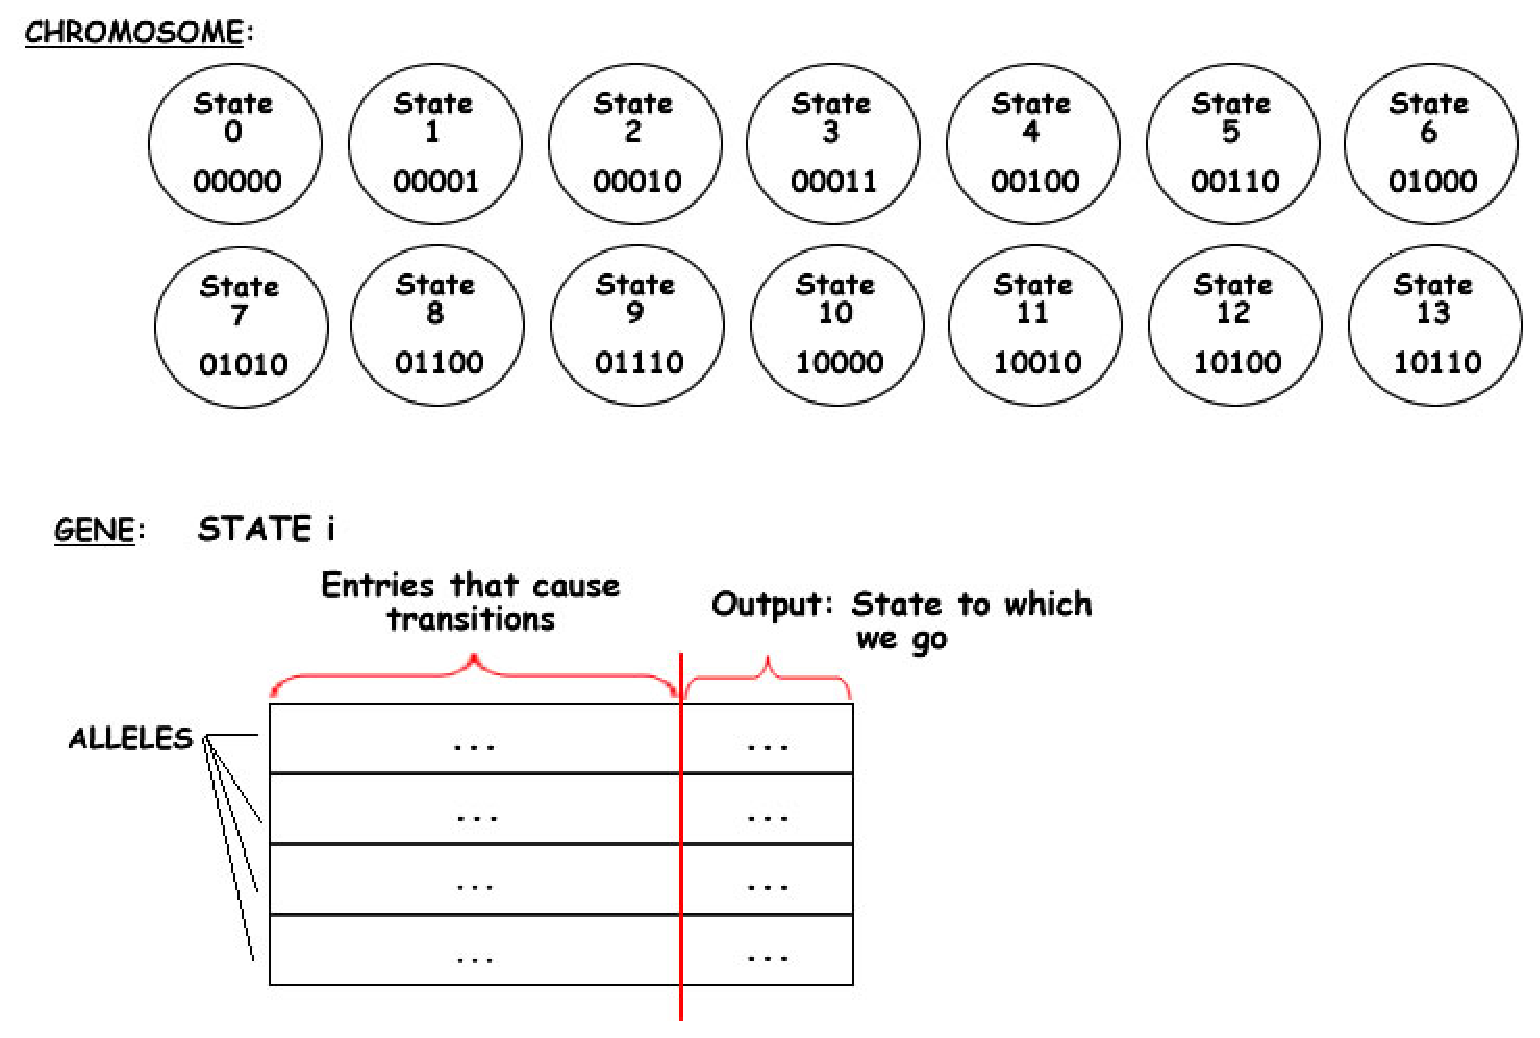
\includegraphics[scale=0.4]{imags/chromosome-fsm.eps}
\caption{Chromosome for the FSM evolution by means of a GA, modelling a state codification.
\label{fig:chromo_fsm}}
\end{center}
\end{figure}

The GA operators applied are as follows. Firstly, we will describe the \textit{fitness function}, since the algorithm performance highly depends on it.
To calculate this function for one individual, the FSM represented in a chromosome is set as the AI of one agent which is placed in a level, and then, it plays for getting the fitness value.
Two different schemes have been implemented:
\begin{itemize}
    \item \textit{mono-seed}: All the individuals are tested in the same level (with the same difficulty) one time, until it passes the level, dies or gets stacked. The length of the level and time to complete it grow with the generations, being easier in the first generations and harder when the algorithm run advances. The aim is to promote the convergence. If the individuals in a generation do not get a good enough fitness, the level length and time remain the same in the next generation.
    \item \textit{multi-seed}: Every individual is tested in 30 levels (in the same difficulty) generated randomly (using different seeds), playing again until pass, die or get stacked. The fitness is computed considering the results of all the plays. The aim of this scheme is: 1) avoid the usual noise \cite{noisyfitness_EVO2012} present in this type of problems (videogames), i.e. it tries to get a fair valuation for an individual, since the same configuration could represent an agent which is very good sometimes and quite bad some others, due to the stochasticity present in every play (just in the agent's behaviour); and 2) get individuals prepared to a wide set of situations in every level and difficulty, since 30 levels should present a high amount of different scenarios and configurations.
\end{itemize}

Thus, there is a \textit{generic fitness} which has as restriction completely finish the level to be set to positive. On the contrary, individuals that have not finished the level start from the lowest fitness possible and their negativity is reduced according the behaviour during the level run. This generic fitness is a weighted aggregation based in the next values:
\begin{itemize}
\item {\em marioWinner}: is set to 1 if the agent finish the level.
\item {\em marioSize}: 0 if the agent is small, 1 if it is Big, and 2 if it is Fire.
\item {\em numKilledEnemies}: as the name suggest, is the number of killed enemies by the agent.
\item {\em numTotalEnemies}: number of total enemies during the level.
\item {\em cells}: number of cells passed by the agent.
\item {\em remainingTime}: time to finish the level.
\item {\em timeSpent}: time spent by the agent.
\item {\em coinsGathered}: number of gathered coins.
\item {\em totalCoins}: total coins appeared in the level.
\item {\em numCollisions}: number of times the agent has bumped with an enemy.
\item {\em numGatheredPowerUps}: number of mushrooms or flower the agent has picked up.
\item {\em causeOfDeath}: in case the agent is dead, this value is also taken into account in the fitness computation.
\end{itemize}

This fitness is considered as the result of the evaluation for the individuals in the mono-seed approach, meanwhile multi-seed considers a {\em hierarchical fitness}, where the population is ordered according the next criteria: 
First, taking into account the percentage of levels where the individuals have been stacked or fallen from a cliff. Then, they are ordered considering the average percentage of levels completed. Finally, the individuals are ordered by the average generic fitness obtained in the levels.

The {\em selection mechanism} considers the best individual and a percentage of the best ones, selected by tournament according to their fitness (generic or hierarchical, depending on the approach). Thus, when comparing two individuals in the multi-seed scheme, three values are considered in cascade: percentage of levels where the agent has been stacked or fallen in a gap, percentage of levels completed, and generic fitness.
The percentage of individuals to consider as parents follows to schemes: in mono-seed it is low at the beginning and will be increased when the number of generations grows; in multi-seed it is constant.

{\em Crossover} is performed considering the best individual of the present generation as one of the parents, and one of the individuals with positive fitness as the other parent. They generate a number of descendents which depends on the percentage of population to complete with the crossover. If there are not enough parents, we select the `less worse' individuals of those with negative fitness.
A uniform crossover has been used, i.e. each gene is randomly selected from one of the two parents.


The {\em Mutation operator} is slightly different from the usual one: after selecting a percentage of individuals to be mutated, various genes in each of these individuals are randomly selected to be mutated. Mutation is performed by randomly changing the output state for an input in the table.

Regarding the {\em replacement} to form the new population, there is a $1-elitism$ mechanism, so the best individual survives. The rest of the population is composed by the offspring generated in the previous generation, which was a percentage of the global population, and the rest of individuals being random ones, in order to increase the diversity. 
The percentage defined, in fact, is related to the number of random individuals, which is the complementary to the percentage of the generated offspring. This value is reduced with the generations in the mono-seed approach, as stated some paragraphs above. The aim is getting a high diversification factor in the first generations, i.e. an exploration phase, and reduce this factor when the best solutions arise (in some generations), changing to an exploitation phase. In multi-seed approach the percentage remains constant (quite small) because the fitness is much more representative of the individuals' quality, so the exploration has a lower significance.

%%%%%%%%%%%%%%%%%%%%%%%%%%%%%  EXPERIMENTS %%%%%%%%%%%%%%%%%%%%%%%%%%%%%%%%

\section{Experiments and Results}
\label{sec:experiments}

In order to test the approaches, several experiments have been conducted.
The initial aim was to find good enough agents for completing any level in any difficulty, but previously it was necessary to perform a hard fine-tuning stage (systematic experimentation), where several different values for the parameters of the algorithm were tested, searching for the best configuration. In addition, a wide analysis on the influence of these parameters was done, due to the difficulties that the algorithms found from level 5 in advance, as will be described in the next paragraphs.

It is important to remark that a single play of an agent could spend around 40-50 seconds on average (it depends on the level length and difficulty), because it must be played in real-time, not simulated. That means that a single evaluation for one individual in the multi-seed approach (30 plays) could take around 25 minutes in some levels. 

Moreover, when the experiments were conducted, it could be noticed than the most difficult levels strongly limited the algorithmic behaviour of the approaches, making it hard to converge and even ending the execution abruptly.
In addition to the high computational cost (one run may take several days), there was a problem with the structure that stores the FSM of the individuals, since it is huge (in memory terms) and grows exponentially during the run (new inputs and outputs are added to the tables in crossovers), so in levels higher than 4, the program frequently crashes.


% -------------------------------------------------------------------
\subsection{Mono-seed approach}

All these experiments were performed on a Phenom II X4 925 with 16GB RAM.
The main problem arose initially in levels higher than 5, where a stack overflow error happened. Thus, the global FSM structure implementation was redesigned to an optimal one, letting to evolve agents in all the possible levels, but with a shorter number of generations than recommended.

The parameter analysis yielded the best configuration for the GA, whose values are presented in Table \ref{tab:params_monoseed}.

\begin{table} [htbp]
\centering
{\footnotesize
\begin{tabular}{|l|l|}
\cline{2-2}
\multicolumn{1}{l|}{} & Optimal value \\ 
\hline
Population size & 1000 (difficulty 0) \\ 
Number of generations & 30 (difficulty 0) \\ 
Crossover percentage & 95\% \\ 
Mutation percentage & 2\% (individuals)\\ 
Mutation rate & 1\% (genes) \\ 
Percentage of random individuals & 5\% (decreased with the generations) \\
Fitness function & generic (aggregation) \\
\hline
\end{tabular}
}
\caption{Optimal parameter values for mono-seed approach.
\label{tab:params_monoseed} }
\end{table}

The values in the table show that a small number of generations is required to get a competent agent in difficulty level 0, along with a population size quite high since every individual is just test once in this approach, so it is needed to ensure the evolution, even considering that none of the individuals may not complete a level. In that cases, some other generations are run to improve them and give another step in the evolution process.
The population study is shown in Figure \ref{fig:population_monoseed}.

\begin{figure}
\begin{center}
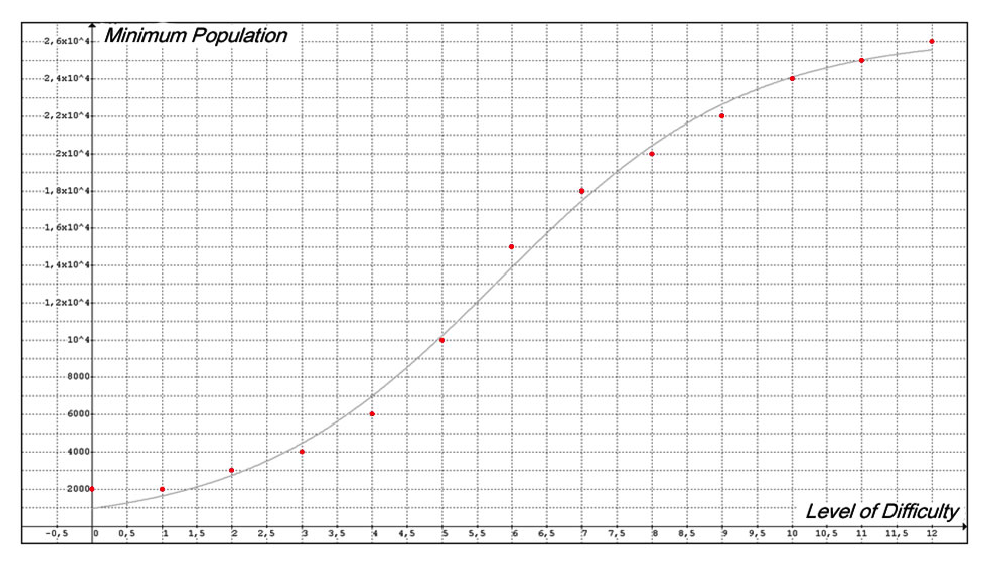
\includegraphics[scale=0.6]{imags/population_monoseed.eps}
\caption{Population size recommended for each difficulty level in mono-seed approach.
\label{fig:population_monoseed}}
\end{center}
\end{figure}

Figure \ref{fig:time_memory_monoseed} presents the requirements in computation time and memory that a complete evolution (run of the algorithm) needed in every difficulty level. 

\begin{figure}
\begin{center}
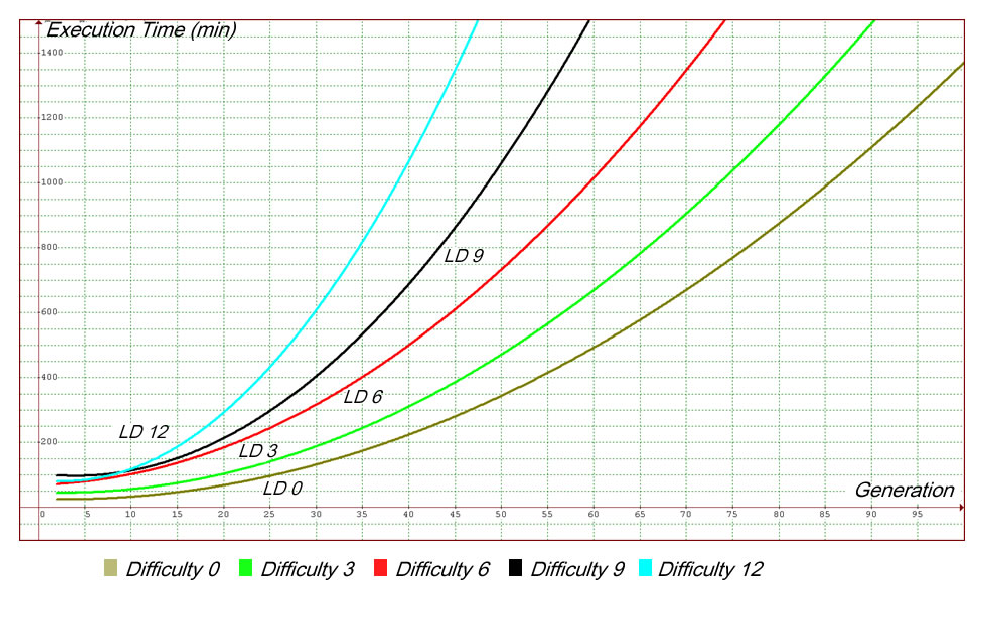
\includegraphics[scale=0.5]{imags/comp_time_monoseed.eps}
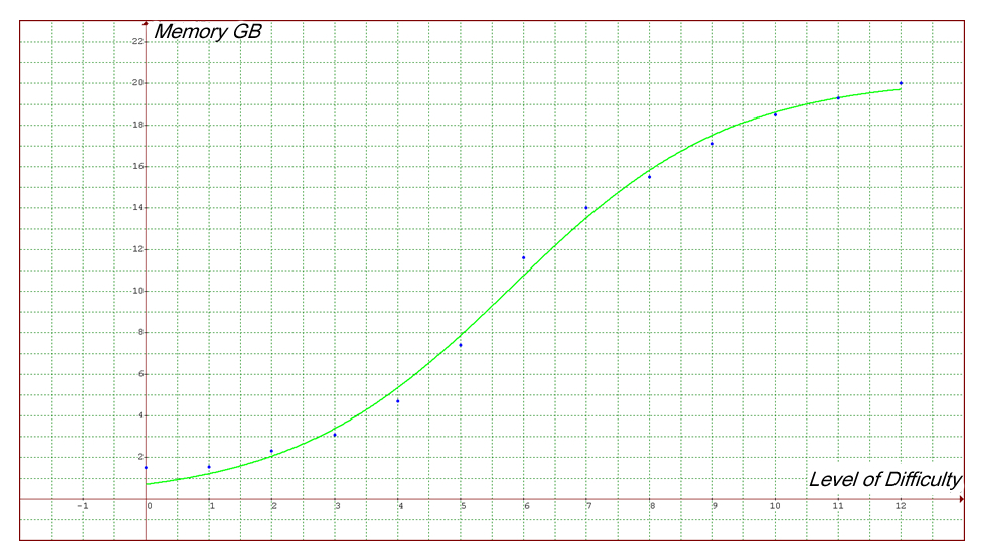
\includegraphics[scale=0.5]{imags/memory_monoseed.eps}
\caption{Execution time (in minutes) and required memory (GB) for mono-seed approach.
\label{fig:time_memory_monoseed}}
\end{center}
\end{figure}

%\begin{figure}
%\begin{center}
%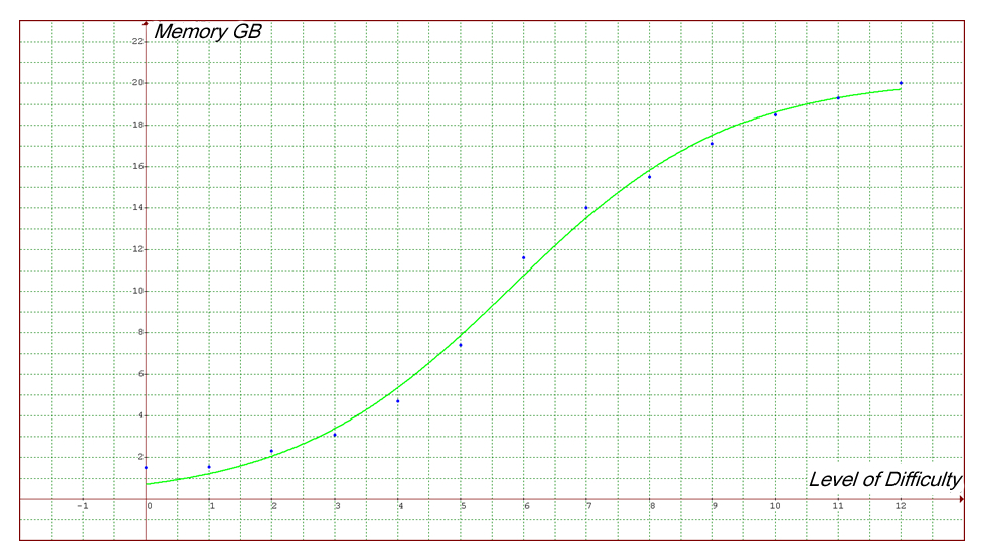
\includegraphics[scale=0.6]{imags/memory_monoseed.eps}
%\caption{Required memory for mono-seed approach.
%\label{fig:population_monoseed}}
%\end{center}
%\end{figure}

The fitness evolution (in difficulty 0) can be seen in Figure \ref{fig:maxfitness_monoseed}, where the maximum fitness value and the number of individuals with positive fitness (required to perform the crossover) are plotted. 

\begin{figure}
\begin{center}
\includegraphics[scale=0.27]{imags/max_fitness_monoseed.eps}
\caption{Maximum fitness in every generation, along with the number of individuals with positive fitness in mono-seed approach. Difficulty level 0.
\label{fig:maxfitness_monoseed}}
\end{center}
\end{figure}

It can be seen that the fitness grows with the generations, as expected in a GA, and there are always enough individuals with positive fitness to assure the offspring generation.

The agents obtained with this approach are very good for the specific level (seed) and difficulty which were set during the optimization process. However their behaviour is quite bad when the level changes the seed or the difficulty, but not the length, since it grows with the generations, as commented in Section \ref{sec:FSMagent}.


% -------------------------------------------------------------------
\subsection{Multi-seed approach}

Due to the problems of the previous experiments, these were conducted on a better computer, an Intel Core i7-920 processor with 32GB RAM.
However the memory problem still remained, so the number of states where reduced to 12, by deleting those considered as non-useful (in Table \ref{tab:FSMstates}): State 8 (no action is done) and State 11 (Mario jumps and crouch, since these actions are not possible simultaneously in this implementation of Infinite Mario).
With this change, it was possible optimizing competent agents from difficulty levels 0 to 4, which are, in turn, enough for the GamePlay competition.

As previously stated, in this approach, every individual is evaluated in 30 different levels: with different random seeds and level type (exterior, subterranean or castle), but with the same length and associated difficulty.

Moreover, in order to get a better computation time, we profited the architecture of the machine, so the fitness evaluation was divided in four parallel threads (four levels at a time), getting an improvement of around four times.

The optimal values for this approach are shown in Table \ref{tab:params_multiseed}.

\begin{table} [htbp]
\centering
{\footnotesize
\begin{tabular}{|l|l|}
\cline{2-2}
\multicolumn{1}{l|}{} & Optimal value \\ 
\hline
Population size & 2000 (difficulty 4)\\ 
Number of generations & 500 (difficulty 4)\\ 
Crossover percentage & 95\% \\ 
Mutation percentage & 2\% (individuals)\\ 
Mutation rate & 1\% (genes)\\ 
Percentage of random individuals & 5\% (constant)\\ 
Fitness function & hierarchical \\
\hline
\end{tabular}
}
\caption{Optimal parameter values for multi-seed approach.
\label{tab:params_multiseed} }
\end{table}

These values show a number of generations smaller than in mono-seed approach for difficulty level 4, which was set to 6000, since the individuals here are evaluated in 30 different levels against just one in that approach, so the adaptation is much more higher and thus, it is not necessary to have a very high amount of individuals.

However, the time expended and memory required are even higher than before, as it can be seen in Figure \ref{fig:time_memory_multiseed}, which shows the analysis of memory and computing time consumed in the evolution until difficulty 4. 

\begin{figure}
\begin{center}
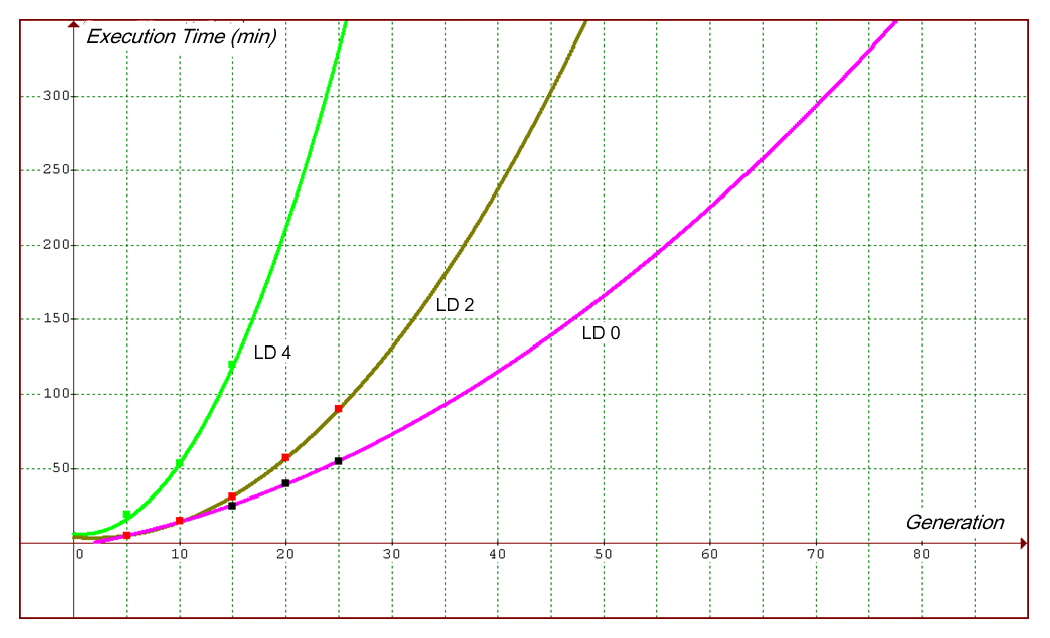
\includegraphics[scale=0.47]{imags/comp_time_multiseed.eps}
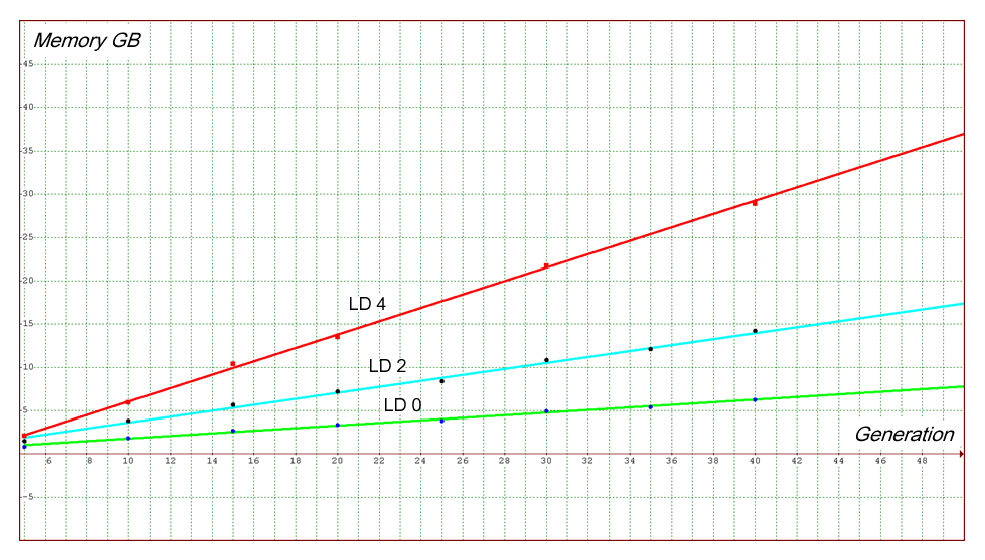
\includegraphics[scale=0.5]{imags/memory_multiseed.eps}
\caption{Execution time (in minutes) and required memory (GB) for multi-seed approach.
\label{fig:time_memory_multiseed}}
\end{center}
\end{figure}

%\begin{figure}
%\begin{center}
%\includegraphics[scale=0.2]{imags/max_fitness_monoseed.eps}
%\caption{Maximum fitness in every generation, along with the number of individuals with positive fitness in *** mono-seed approach ***. Difficulty level 0.
%\label{fig:maxfitness_multiseed}}
%\end{center}
%\end{figure}

However, the agents obtained with multi-seed approach are capable of complete (almost) any level in every difficulty for which they have been optimized.

Some examples of the obtained evolved FSM-based agents can be seen in action (in a video) from the next urls:
\begin{itemize}
    \item \textit{Difficulty level 1 (completed)}: \url{http://www.youtube.com/watch?v=6Pj6dZCE070}
    \item \textit{Difficulty level 2 (completed)}: \url{http://www.youtube.com/watch?v=gtfuY-L0WDA}
    \item \textit{Difficulty level 3 (completed)}: \url{http://www.youtube.com/watch?v=qQVQ43sWwYY}
    \item \textit{Difficulty level 12 (stacked)}: \url{http://www.youtube.com/watch?v=zNGfBApX7sk}
\end{itemize}

The last one was evolved for some generations (not all the desired) in that level of difficulty, due to the commented problems, so it cannot complete this hard level in the simulator. However, as it can be seen, it is quite good in the first part of the play. Thus, if we could finish the complete evolution process in this difficulty level we think the agent could complete any possible level.

%LT -> Tipo de escenario. Escenario 0: superficie, escenario 1: subterr�neo, escenario 2: castillo
%LD -> Dificultad del nivel. Valores entre 0 y 12
%LL -> Longitud del nivel. Valor de 26 a $2^(31)-1$
%LS -> Semilla aleatoria de generaci�n de nivel. Valor de 0 a $2^(31)-1$
%


\section{Conclusions and Future Work}
\label{sec:conclusions}

In this work, two different approaches for evolving, by means of Genetic Algorithms (GAs), agents which play Super Mario Game have been proposed and analyzed. They have been implemented using Finite State Machine (FSM) models, and considering different evaluation schemes, with a mono-seed and a multi-seed approach for evaluating the individuals, and two different fitness functions.
Both algorithms have been tested inside a simulator named Mario AI, based in the so-called Infinite Mario Bros, and which was implemented for the Mario AI Competition. The proposed agents were devoted, in principle to participate in the GamePlay Track of that competition.

Several experiments have been conducted to test the algorithms and a deep analysis has been performed in each case, in order to set the best configuration parameters for the GA. However some problems have arisen such as the high memory requirements, which have made it difficult to complete the optimization process in several cases.

However, very competent agents have been obtained for the difficulty levels 0 to 4 in both approaches, which are, in turn, enough for the Game Play competition.

In the comparison between the approaches, mono-seed can yield excellent agents for the level where they were `trained' (evolved), having a quite bad behaviour in a different level. Multi-seed takes much more computational time and has higher resource requirements, but the agents it yields are very good playing in any level of the considered difficulty (in the evolution). All these agents play much better than an expert human player and can complete the levels in a time impossible to get for the human.

Since this is a novel research scope for the authors, several future lines of work are opened, starting with the resolution of the commented memory problem. A redesign of the GA's chromosome structure could be useful in this sense.
We definitely think that if it is possible to completely evolve a population of agents with the multi-seed scheme, the best of them might complete any level.
Moreover, some other algorithmic proposals should be tested, such as a reduction in the number of individuals in the population, along with a change in the selection, crossover and mutation mechanisms to control the required balance between exploration and exploitation in GAs.

Another line of research could be the consideration of a high-level expert knowledge in the FSM. For instance each state should be based in principles proposed by \cite{SuperMario_rulebased}. That means the agents should be not designed according a fixed set of states, but the specific necessities it should to solve. This solution could reduce the search space and increase the possibility to solve harder levels.

\section*{Acknowledgements}
This work has been supported in part by the P08-TIC-03903 project awarded by the Andalusian Regional Government, the FPU Grant 2009-2942 and the TIN2011-28627-C04-02 project, awarded by the Spanish Ministry of Science and Innovation.

\bibliographystyle{splncs}
%\bibliography{paperMario}

\begin{thebibliography}{00}

\bibitem{EAs_Back96}
B\"ack, T., \emph{Evolutionary algorithms in theory and practice}, Oxford University Press, 1996.

\bibitem{SuperMario_Astar}
R. Baumgarten, \emph{Mario AI A* agent},
http://www.doc.ic.ac.uk/~rb1006/projects:marioai.

\bibitem{SuperMario_rulebased}
Bojarski, S., Bates-Congdon, C., \emph{REALM: A Rule-Based Evolutionary Computation Agent that Learns to Play Mario}. In: Proceedings of the 2011 IEEE Symposium on Computational Intelligence and Games (CIG 2011), IEEE Press, pp. 83--90, 2011. 

\bibitem{FSM_Booth}
Booth, T.L., \emph{Sequential Machines and Automata Theory}, John Wiley and Sons, Inc., New York, 1st edition, 1967.

%\bibitem{ControllingBot_CEC2010}
%Esparcia-Alc{\'a}zar A I, Mart�nez-Garc\'{\i}a A I, Mora A M, Merelo J J, Garc\'{\i}a-S{\'a}nchez P. Controlling bots in a first person shooter game using genetic algorithms. In \emph{Proc. 2010 IEEE Congress on Evolutionary Computation (CEC 2010)}, July 2010, pp. 1--8.

\bibitem{GAs_Goldberg89}
Goldberg D.E., Korb B., Deb K., \emph{Messy genetic algorithms: motivation, analysis, and first results}, Complex Systems, 3(5), pp. 493--530, 1989.

\bibitem{potfields_starcraft}
Hagelb\"ack, J., \emph{Potential-Field Based navigation in StarCraft}. In: Proceedings of the 2012 IEEE Symposium on Computational Intelligence and Games (CIG 2012), IEEE Press, pp. 388--393, 2012. 

\bibitem{optimalRTS}
Jang, S.H., Yoon, J.W., Cho, S.B., \emph{Optimal strategy selection of non-player character on real time strategy game using a speciated evolutionary algorithm}. In: Proceedings of the 5th IEEE Symposium on Computational Intelligence and Games (CIG'09), IEEE Press, pp. 75--79, 2009.

\bibitem{laird2001using}
Laird, J.E, \emph{Using a computer game to develop advanced AI}.
  Computer, 34(7), pp. 70--75, 2001.

\bibitem{Pac-MAnt_CIG2010}
Mart�n, E., Mart�nez, M., Recio, G., Saez, Y., \emph{{Pac-mAnt}: Optimization based on ant colonies applied to developing an agent for Ms. Pac-Man}. In Proc. 2010 IEEE Conference on Computational Intelligence and Games (CIG 2010), IEEE Press, pp. 458--464, 2010.

\bibitem{cooperativebots_CIG2010}
Mora, A.M., Moreno, M.A., Merelo, J.J., Castillo, P.A., Garc�a-Arenas, M.I., Laredo, J.L.J., \emph{Evolving the cooperative behaviour in {Unreal}\texttrademark~ bots}. In Proc. 2010 IEEE Conference on Computational Intelligence and Games (CIG 2010), IEEE Press, pp. 241--248, 2010.

\bibitem{noisyfitness_EVO2012}
Mora, A.M., Fern�ndez-Ares, A., Merelo, J.J., Garc�a-S�nchez, P., \emph{Dealing with noisy fitness in the design of a RTS game bot}. In Proc. Applications of Evolutionary Computing: EvoApplications 2012, LNCS, vol. 7248, Springer, pp. 234--244, 2012.

\bibitem{SuperMario_playerexperience}
Pedersen, C., Togelius, J., Yannakakis, G., \emph{Modeling Player Experience in Super Mario Bros}. In Proc. 2009 IEEE Symposium on Computational Intelligence and Games (CIG'09), IEEE Press, pp 132--139, 2009.

\bibitem{MTCS_PacMan}
Pepels, T., Windans, H.M., \emph{Enhancements for Monte-Carlo Tree Search in Ms Pac-Man}. In Proc. 2012 IEEE Conference on Computational Intelligence and Games (CIG 2012), IEEE Press, pp. 265--272, 2012.

\bibitem{tactics_evolutionary_learning}
Ponsen, M., Munoz-Avila, H., Spronck, P., Aha, D.W., \emph{Automatically generating game tactics through evolutionary learning}. AI Magazine, 27(3), pp. 75--84, 2006.

\bibitem{SuperMario_levelgeneration}
Shaker, N., Nicolau M., Yannakakis, G.N., Togelius, J., O\textquoteright neill, M., \emph{Evolving Levels for Super Mario Bros Using Grammatical Evolution}. In Proc. 2012 IEEE Symposium on Computational Intelligence and Games (CIG 2012), IEEE Press, pp 304--311, 2012.

\bibitem{Agent_Smith_CEC2009}
Small, R., Bates-Congdon, C. \emph{Agent {S}mith: Towards an evolutionary
  rule-based agent for interactive dynamic games}. In Proc. 2009 IEEE Congress on Evolutionary Computation (CEC'09), pp. 660--666, 2009.

\bibitem{evolutionary_learning-offline}
Spronck, P., Sprinkhuizen-Kuyper, I., Postma, E., \emph{Improving opponent intelligence through offline evolutionary learning}. International Journal of Intelligent Games and Simulation, 2(1), pp. 20--27, 2003.

\bibitem{starcraft_bayesianmodel}
Synnaeve, G., Bessi�re, P., \emph{A Bayesian Model for RTS Units Control applied to StarCraft}. In Proc. 2011 IEEE Symposium on Computational Intelligence and Games (CIG 2011), IEEE Press, pp 190--196, 2011.

\bibitem{SuperMario_Togelius}
Togelius, J., Karakovskiy, S., Koutnik, J., Schmidhuber, J., \emph{Super Mario
  evolution}. In Proc. 2009 IEEE Symposium on Computational Intelligence and Games (CIG'09), IEEE Press, pp 156--161, 2009.

\end{thebibliography}

\end{document}


% VIDEOS:
%
% dif 12 -> stacked: http://www.youtube.com/watch?v=zNGfBApX7sk
% dif 12 (20 seconds): http://www.youtube.com/watch?v=46yK4laTU0E
% dif 3 -> passed: http://www.youtube.com/watch?v=qQVQ43sWwYY
% dif 2 -> passed: http://www.youtube.com/watch?v=gtfuY-L0WDA
% dif 1 -> passed: http://www.youtube.com/watch?v=6Pj6dZCE070
